
A very simple solution was tried first in the project. It consisting of a Mixture of Gaussian model\cite{Gardel} used for segmenting the moving foreground from the background as a binary mask. Then all connected moving objects were found and tracked using a simple tracker.g of the moving objects. This approach was developed and performed good for tracking people moving relatively fast, but worse or not at all for people moving slow and standing still. This approached suffered from problems such as be unable to handle common occlusions when people stand and move too close to each other, especially when doing so from entering to leaving the field of view. To segment persons in such situations required more advanced methods which we tried but never managed to work well enough. Further improvements on this approach were therefore never implemented. The approach also required quite some morphological operations to connect loosely connected components of humans, as seen in figure \ref{fig:bg_success}, or very restrictive limits on minimum area.\\
\\
Using a more sophisticated tracker with prediction and which remembered still, persons even as they became a part of the background, most problems except the severe occlusions could possibly been coped with. Another solution would have been to identify humans and disallow the background model from learning those region, eliminating the disappearances of tracked persons. \\
\\
The algorithm described in \cite{Gardel} was chosen since it was the most recent developed background subtractor in OpenCV, and also the best performing one according to the OpenCV reference manual. 

\vspace{1cm}
\begin{figure}[htb]
	\centering
	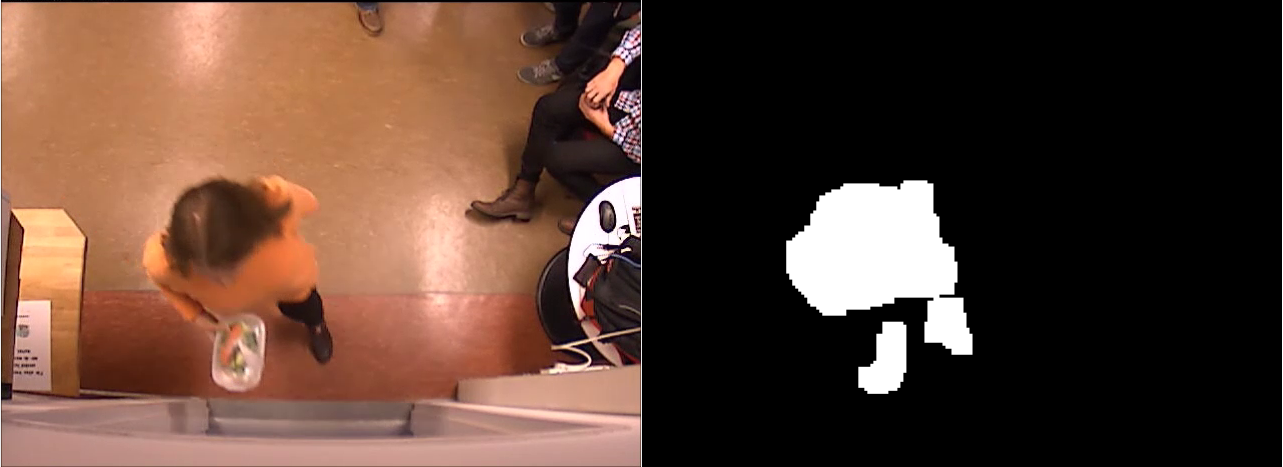
\includegraphics[width=\linewidth]{images/bg_success.png}
	\caption[An example of scattered binary mask of a human from the background model.]{\textit{The left image shows a moving person who is detected by the background subtractor. The right image shows the binary image generated from the left image, illustrating the scattered parts separated due to none-uniform motion.
	}}
	\label{fig:bg_success}  %Skapar referens till figuren
\end{figure}

